\documentclass{article}
\usepackage[utf8]{inputenc}
\usepackage[spanish]{babel}
\usepackage{listings}
\usepackage{graphicx}
\graphicspath{ {images/} }
\usepackage{cite}

\begin{document}

\begin{titlepage}
    \begin{center}
        \vspace*{1cm}
            
        \Huge
        \textbf{Calistenia}
            
        \vspace{0.5cm}
        \LARGE
        
            
        \vspace{1.5cm}
            
        \textbf{Carolina Jiménez Restrepo}\\
        \textbf{c.c 1020470694}
          \\  Grupo 3
         
         \vspace{2.9cm}
         
          profesor: Augusto Enrique Salazar Jimenez
          Curso: Inform´atica II


        \vfill
            
        \vspace{0.8cm}
            
        \Large
        Despartamento de Ingeniería Electrónica y Telecomunicaciones\\
        Universidad de Antioquia\\
        Medellín\\
        Marzo 09 de 2021
            
    \end{center}
\end{titlepage}

\tableofcontents
\newpage
\section{Sección introductoria}\label{intro}
Tenemos el desafío de pasar un objeto que se encuentra en una posición A a una posición B, este desafío consiste en formar una pirámide utilizando dos cartas y con una sola mano. Se desarrollaron unos pasos específicos para lograr cumplir el objetivo, estos pasos serán puestos a prueba por tres personas diferentes para las que no hay un rango ni limite de edad y las cuales no tendrán ningún tipo de conocimiento previo de qué hacer y qué se debe lograr, solo seguirán los pasos propuestos para cumplir nuestro objetivo.

\section{Sección de contenido y desarrollo} \label{contenido}
Lo primero que haremos es conocer los implementos a utilizar, necesitaremos una hoja de papel que este en buen estado, dos tarjetas del mismo tamaño y una superficie plana y lisa. \\
Para comenzar a dar solución a nuestro desafío vamos a conocer cuales son las posiciones o estados A y B. La posición A es el estado inicial, del que vamos a partir, este consiste en tener las dos tarjetas una sobre otra y la hoja de papel sobre ellas cubriéndolas. La posición B es el estado final, al que queremos llegar, ¡es nuestro objetivo! Este consiste en poner las dos tarjetas en forma de pirámide o especie de techo de casa sobre la hoja con una sola mano. \\

Realicé el análisis e intenté  varias veces cumplir el objetivo y diseñe una serie de pasos con la mejor y más especifica manera de lograr llegar a nuestro estado final, los pasos describen que debe hacer una persona partiendo del estado inicial o posición A para llegar al estado final o posición B, estos pasos fueron puestos a prueba por tres personas diferentes, las cuales no  tuvieron un conocimiento previo de que debían hacer, los objetos se pusieron en el estado inicial y se  les compartió una imagen y a otros una hoja con los pasos a seguir.
.
\subsection{Pasos para lograr cumplir el reto}

1. Con una sola mano coger la hoja de la parte inferior y ponerla a un lado de las tarjetas.
 \\2.	Las tarjetas se encuentran una sobre la otra, con una sola mano las cogemos y las mantenemos juntas, una sobre la otra.
\\3.	Con las tarjetas en la mano y juntas las ponemos en posición vertical y las ubicamos sobre la hoja. 
\\4.	Sostenemos las tarjetas de los costados verticales, el dedo pulgar y el anular van en la parte inferior de las tarjetas, el dedo medio se ubica a unos centímetros del anular o en la mitad de las tarjetas en el costado vertical y el dedo índice en la parte superior horizontal. \\
5.	Con el dedo pulgar y anular deslizamos hacia atrás un poco la tarjeta que está en la parte trasera, sosteniendo con el dedo índice que se encuentra en la parte superior las dos tarjetas para que no se suelten. \\
6.	Dejamos que la tarjeta que está en la parte frontal recaída un poco sobre la tarjeta trasera para formar una pirámide o especie de techo de casa. 






\section{Inclusión de imágenes} \label{imagenes}

En las Figuras (\ref{fig:piramide1}), (\ref{fig:piramide2}), se   presentan las imagenes de la solucion del reto contenida en la carpeta images.

\begin{figure}[h]
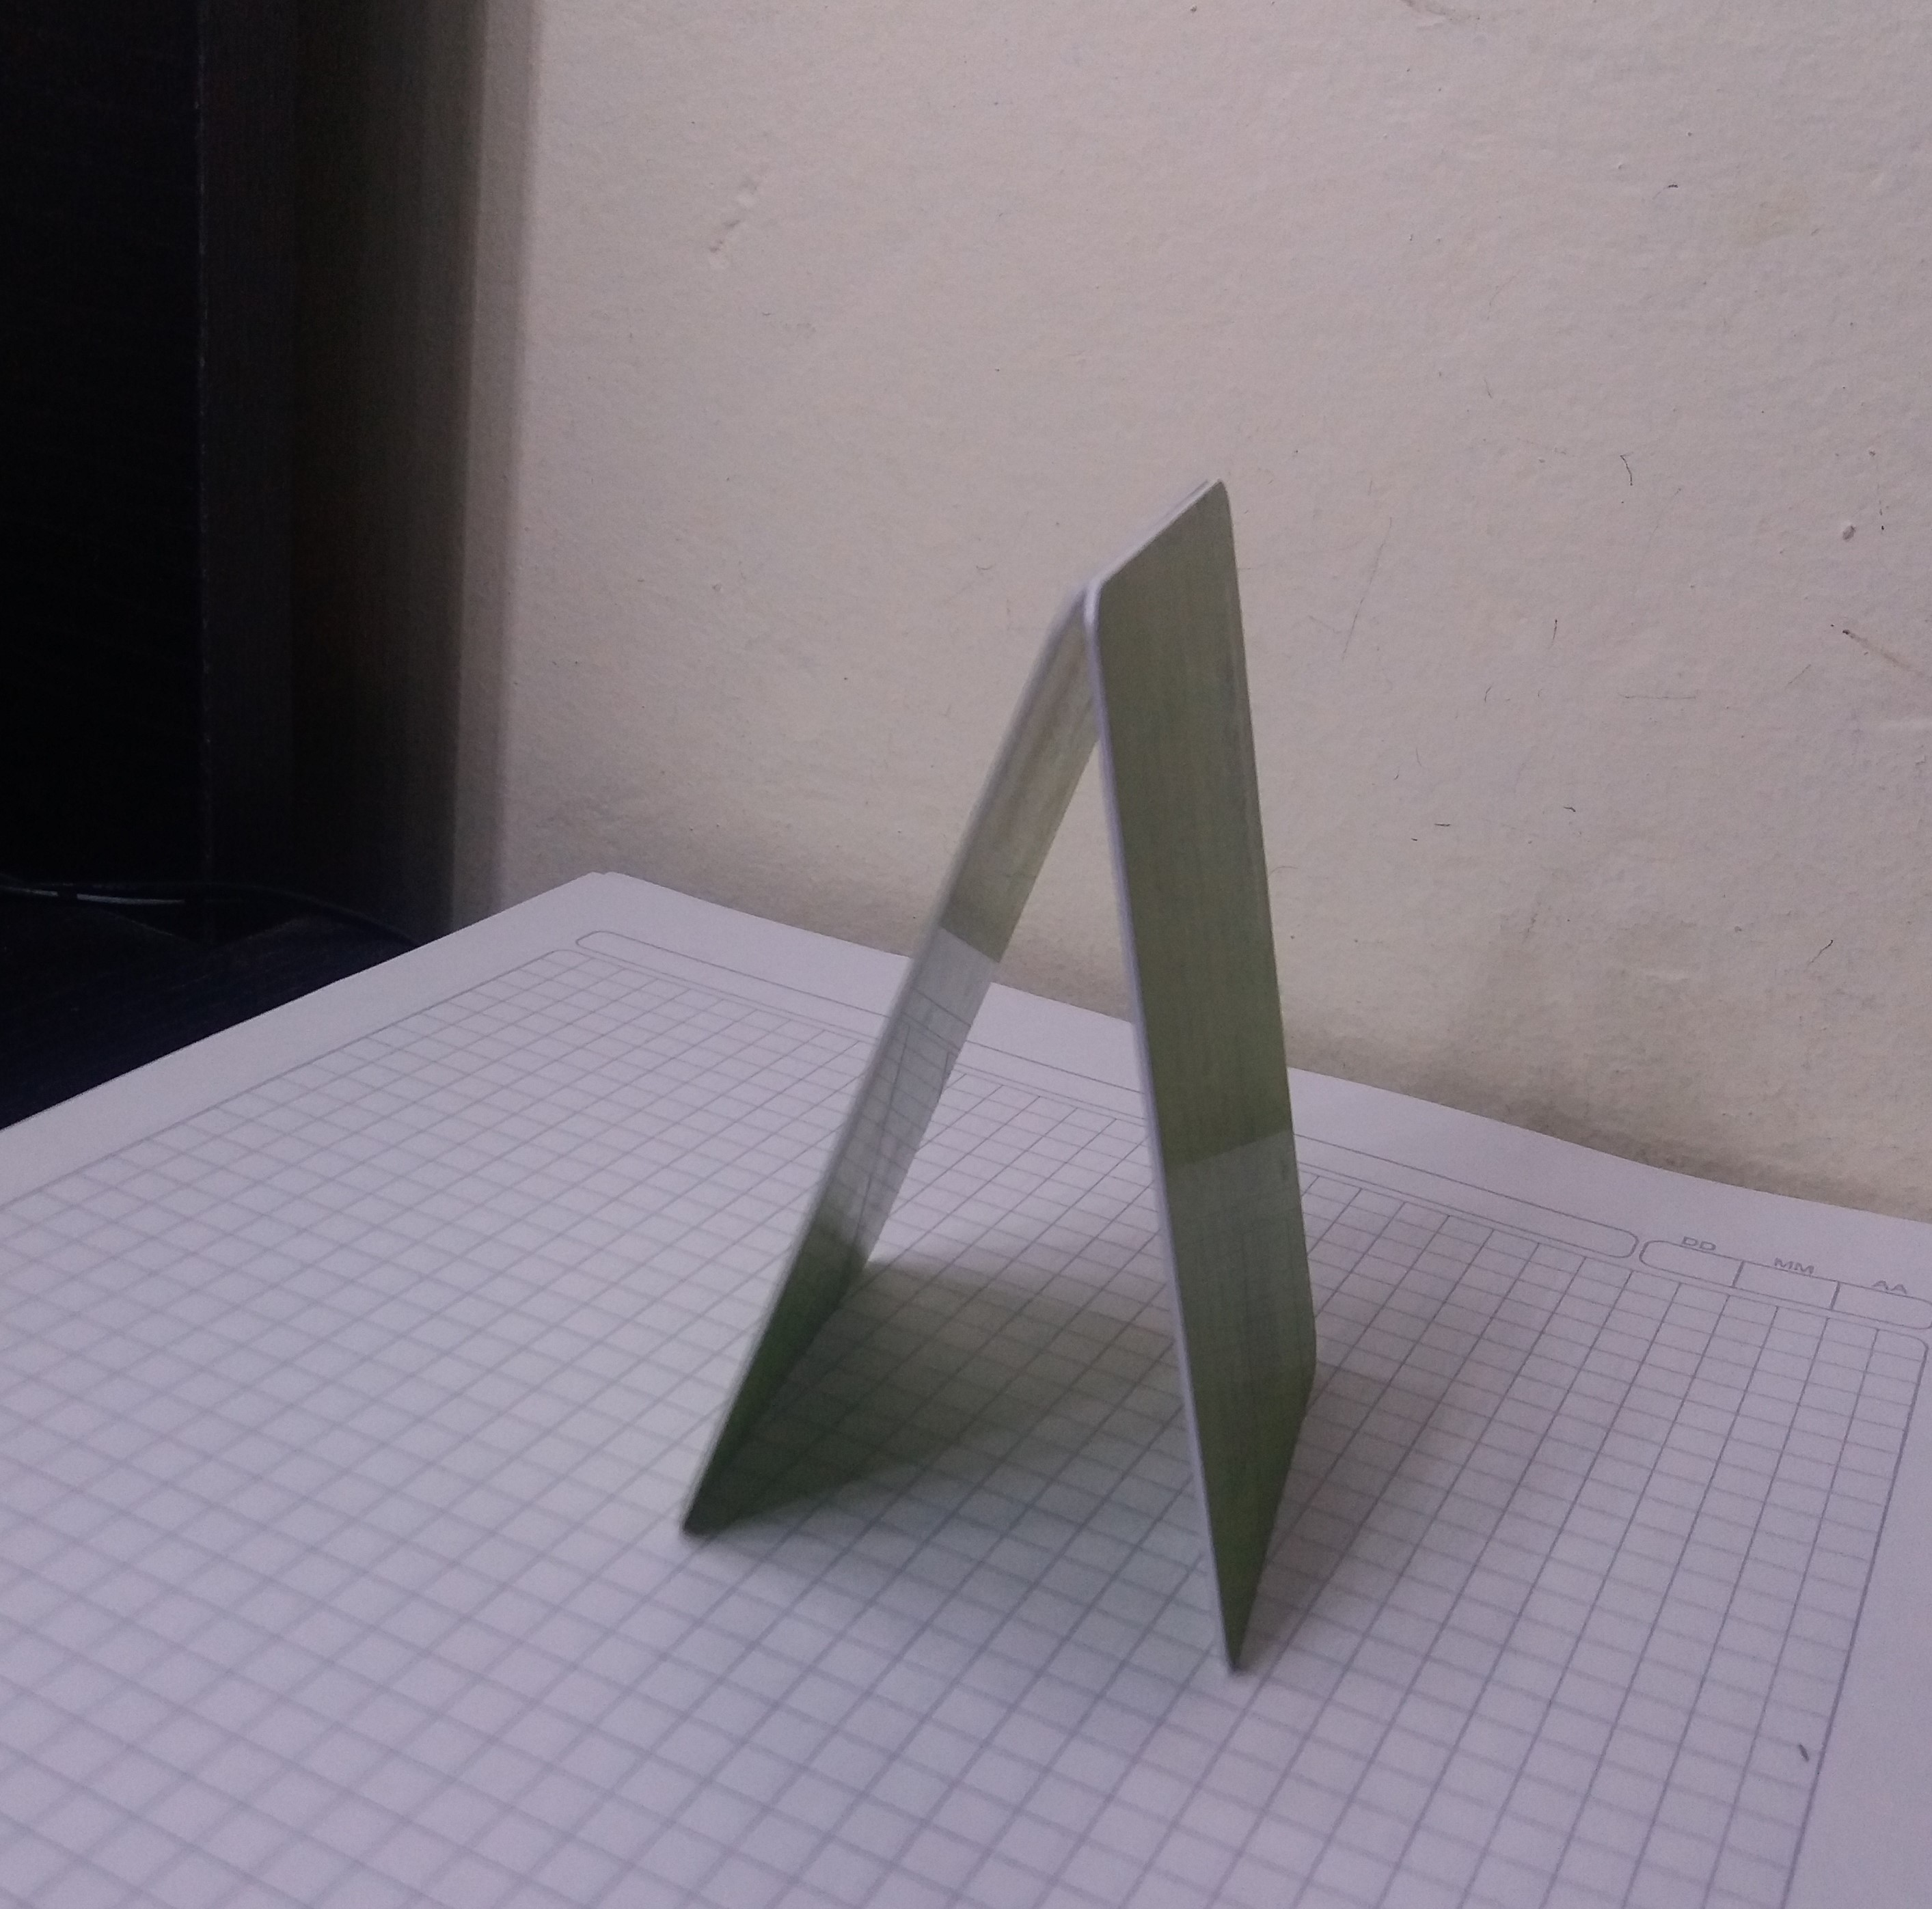
\includegraphics[width=4cm]{piramide1.jpg}
\centering
\caption{}
\label{fig:piramide1}
\end{figure}

\begin{figure}[h]
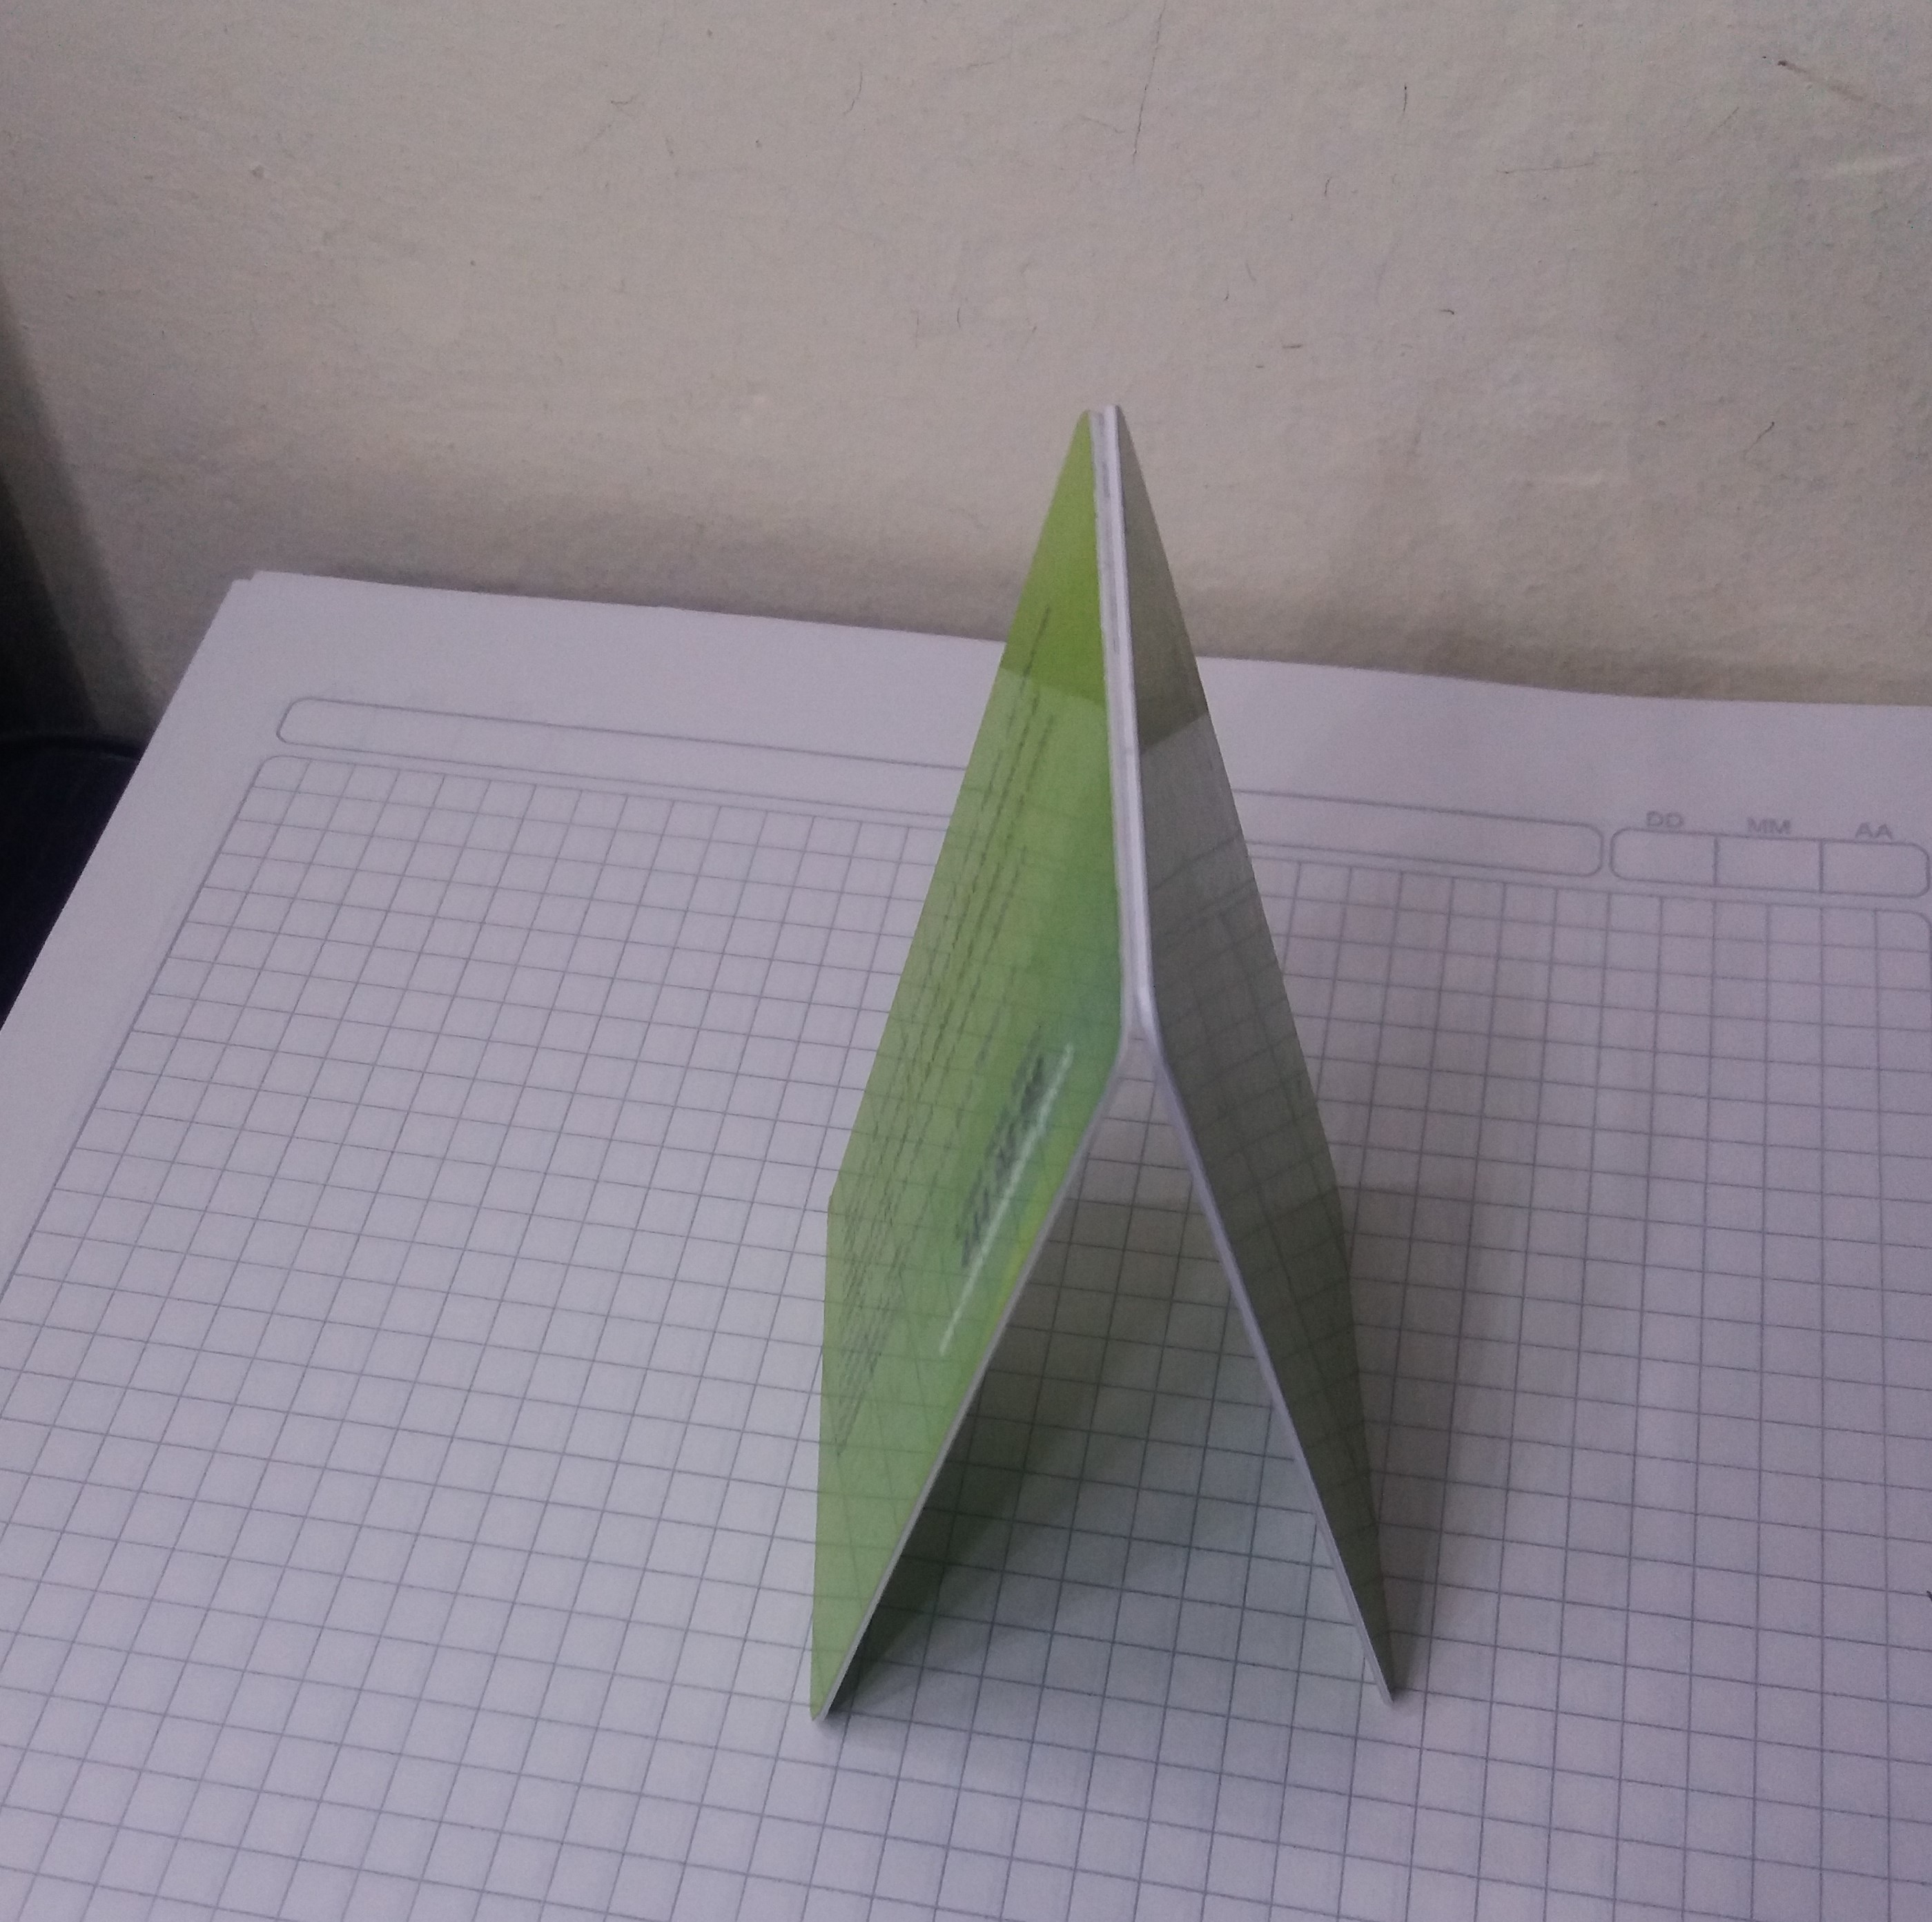
\includegraphics[width=4cm]{piramide2.jpg}
\centering
\caption{}
\label{fig:piramide2}
\end{figure}

.
\section{Sección de conclusiones} \label{contenido}
Al poner a prueba la solución con tres personas, las cuales partieron del estado inicial sin tener ninguna información sobre qué debían hacer, su única guía eran los pasos descritos anteriormente. Notamos que dos de las personas entendieron fácilmente las instrucciones y a una, aunque siguió los pasos, no logró cumplir el objetivo. Esta última persona luego de realizar el ejercicio, manifestó que no tuvo buena comprensión al leer, tuvo poca concentración y afán al aplicar el último paso con el que se lograba dar solución al reto.\\

Con dos de tres personas que lograron cumplir el desafío podemos concluir que los pasos dan la información suficiente para lograr el desarrollo del ejercicio sin tener conocimientos previos, también debemos tener en cuenta que la persona que siga los pasos debe leer detenidamente y tener una buena comprensión de lo que se dice, al igual que conocer el nombre de los dedos de la mano para así facilitar el proceso. Se debe ser muy especifico al realizar los pasos ya que la otra persona no conoce lo que debe lograr, y esto es un trabajo algo difícil que necesita de paciencia y saber que estamos describiendo algo que es desconocido para otros.




\end{document}
